\documentclass[12pt]{report}
\usepackage{graphicx}
\usepackage{scribe_MG}
\usepackage{amssymb}
\usepackage{graphicx}
\usepackage[mathscr]{eucal}
\usepackage[english]{babel}
\usepackage[utf8]{inputenc}  %encodage du fichier
\usepackage[T1]{fontenc}
\usepackage{lmodern}
\usepackage{epstopdf}
\usepackage{array}

\usepackage{placeins}

%% William
\usepackage[colorlinks]{hyperref} % for links
\usepackage{xcolor}             % for color
\usepackage{caption}            % for caption* (without 'Figure 2.n:')
\usepackage{float}              % for H, to place figure HERE!
\usepackage{wrapfig}
\usepackage{tikz}
\usetikzlibrary{arrows}
\usetikzlibrary{positioning}

%% Philippe
\usepackage{amsmath,graphicx}
\newcommand{\widesim}[2][1.5]{
  \mathrel{\overset{#2}{\scalebox{#1}[1]{$\sim$}}}
}

\usepackage{bbm}            % for the indicator function symbol : \mathbbm{1}
\def\R{\mathbb{R}}
\newcommand{\defobj}[1]{\color{red}#1\color{black}{}}
\newcommand{\defmean}[1]{\color{green!70!black}#1\color{black}{}}
\renewcommand{\emph}[1]{\color{violet}#1\color{black}{}}
\DeclareMathOperator{\E}{\mathbb{E}}
\DeclareMathOperator{\Var}{\mathbb{V}\text{ar}}

\newcommand{\sigmaField}{\mathcal{E}}

%% For footnote horizontal spacing :
%% \usepackage{footmisc}
%% \setlength{\footnotemargin}{2mm}

\newcommand\independent{\protect\mathpalette{\protect\independenT}{\perp}}
\def\independenT#1#2{\mathrel{\rlap{$#1#2$}\mkern2mu{#1#2}}} 

\newcommand{\indep}{\ensuremath{\,\bot\!\!\!\bot\,}} %% The symbol for independent
\newcommand{\notindep}{\indep\!\!\!\!\!/\,\,\,}

\newtheorem{remark}{Remark}[section]
\newtheorem{example}{Example}[section]
\newtheorem{property}{Property}[section]

\newcommand{\Bern}{\text{Bern}}
\newcommand{\Bin}{\text{Bin}}


\begin{document}
\coursetitle{IFT 6269: Probabilistic Graphical Models}
\semester{Fall 2017}
\lecturer{Simon Lacoste-Julien} \scribe{Philippe Brouillard and Tristan Deleu}
\lecturenumber{3} \lecturedate{September 12}

\maketitle

\textbf{Disclaimer:} These notes have only been lightly proofread.

\section{Parametric Models}

\subsection{Family of distributions}
A \emph{parametric model} is a family of distributions that is defined by a fixed finite number of parameters.\footnote{We will see later in the class \emph{non-parametric models}, which basically means that the number of parameters is (potentially) infinite. These models are usually fit from data with a number of (effective) parameters growing with the size of training data.}

A \defobj{family of distributions} is formally defined as follows:
\defmean{$$ \mathcal{P}_\Theta = \{ p_\theta (\cdot ; \theta) \mid \theta \in \Theta \} $$}
where $  p_\theta (\cdot ; \theta) $ is the possible pmf or pdf (understood from context) depending on the parameter $ \theta $ and $ \Theta $ is the set of all valid parameters.\footnote{Using $ p_\theta (x ; \theta) $ instead of $ p_\theta (\cdot ; \theta) $ would be an abuse of notation since $ p_\theta (x ; \theta) $ is only a scalar for a specific $ x $ and not a pmf/pdf.}

The support of distribution $ \Omega_{X} $ is usually fixed for all $ \theta $. For example, the support of a distribution modelling a coin flip could be $ \Omega_{X} = \{ 0,1 \}$. Similarly, for the gamma distribution, the support is $ \Omega_{X} = \lbrack 0, + \infty \lbrack$.

\subsection{Notation}
To indicate that a random variable is distributed as a known distribution, we use the symbol ''$ \sim $''. For example, to indicate that the random variable $ X $ is distributed as a Bernoulli distribution of parameter $ \theta $, we would write:
$$ X \sim \Bern (\theta) $$
This notation is a shorthand for:
$$ p(x ; \theta) = \Bern (x ; \theta) $$
where $p(x ; \theta)$ represents the pmf for $X$, and $\Bern (x ; \theta)$ indicates that we refer to the pmf (on $x$) for the Bernouilli distribution.

To take another example, if the random variable $ X $ is distributed as a Normal distribution with parameters $ \mu $ and $ \sigma^{2} $, we would write:
$$ X \sim \mathcal{N} (\mu, \sigma^{2}) $$
that is similar to say that it has a pdf (as now $X$ is a continuous R.V.):
$$ p(x ; (\mu, \sigma^{2})) = \mathcal{N} (x \mid \mu, \sigma^{2}) $$

\subsection{The Bernoulli distribution}
The \emph{pmf} of a \defobj{Bernoulli random variable} $ X $ is given as follows:

\defmean{$$ p(x \mid \theta) = \theta^x (1 - \theta)^{1 - x} $$}

The support of the distribution is $ \Omega_{X} = \{ 0, 1\} $ and the space of the parameters is $ \Theta = \lbrack 0, 1 \rbrack$. From the pmf, we can see that $ P \{ X = 1 \mid \theta \} = \theta $.\footnote{Note that instead of $ \theta $, $ p $  is also often used as a parameter for the Bernoulli and the Binomial distribution.}

The expected value and the variance of a Bernoulli random variable $ X $ are:
$$ \mathbbm{E}\lbrack X \rbrack = \theta $$
$$ \Var\lbrack X \rbrack = \theta (1 - \theta)$$

We can see from the figure below that the variance is at its highest point when $ \theta = 1/2 $.

\begin{figure}[H]\centering
  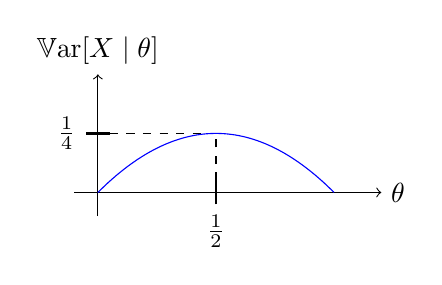
\begin{tikzpicture}[scale=3]
    \draw[->] (-0.1,0) -- (1.2,0) node[right] {$ \theta $};
    \draw[->] (0,-0.1) -- (0,0.5) node[above] {$ \Var \lbrack X \mid \theta \rbrack $};
    \draw[line width=1pt] (-0.05,0.25) -- (0.05,0.25) node[left=0.3cm] {$ \frac{1}{4} $};
    \draw[line width=1pt] (0.5,-0.05) -- (0.5,0.05) node[below=0.3cm] {$ \frac{1}{2} $};
    \draw[dashed] (0.05,0.25) -- (0.5, 0.25);
    \draw[dashed] (0.5,0.05) -- (0.5, 0.25);
    \draw[scale=1,domain=0:1,smooth,variable=\x,blue] plot ({\x},{-(\x)*(\x) + (\x) });
  \end{tikzpicture}
\end{figure}


Intuitively, the Bernoulli distribution models a situation where there are only two possible outcomes: either a success or a failure. The classical example is a coin flip: if getting a head is a success, $ X $ will equals 1. In this case, the parameter $ \theta $ would be the probability to get a head.

\subsection{The Binomial distribution}
A \defobj{binomial distribution} $ \Bin (n, \theta)$ can be defined as the sum of $ n $ \emph{independent and identically distributed} (i.i.d.) Bernoulli random variables with parameter $ \theta $. Formally:

\begin{itemize}
  \item[] Let $ X_{i} \widesim{iid} \Bern (\theta) $ \footnote{ Implicitly, $ X_{i} $ refers to $ X_1,... ,X_n$  }
  \item[] Let $ X = \sum_{i = 1}^{n} X_{i} $ 
  \item[] then we have that $ X \sim \Bin(n, \theta)$
\end{itemize}

The support of the distribution is $ \Omega_{X} = \{ 0, 1, ..., n \} $ and the space of the parameters is $ \Theta = \lbrack 0, 1 \rbrack$.

The \emph{pmf} is given as follows:

\defmean{ $$ p(x; \theta) = \binom nx \theta^x (1 - \theta)^{n - x} $$ }

The term \defobj{$ \binom nx $} is equal to the number of ways to get $ x $ successes out of $ n $ trials. Formally, this is defined as follow:

\defmean{ $$ \binom nx \triangleq \frac{n!}{x! (n - x)!} $$ }

As for the term $ \theta^x (1 - \theta)^{n - x} $, we can notice that it is the product of the pmf of $ n $ Bernoulli random variables, since: 
$$ \theta^x (1 - \theta)^{n - x} = \theta^{{\Sigma x_i}} (1 - \theta)^{\Sigma (1 - x_i)} = \prod_{i=1}^{n} \Bern(x_i; \theta) $$

The expected value and the variance of a Binomial random variable X can be deduced from
the Bernoulli's expected value and variance, since $ X = \sum_{i = 1}^{n} X_{i} $ :
$$ \mathbbm{E}\lbrack X \rbrack = \sum_i \mathbbm{E}\lbrack X_i \rbrack = n \theta $$
$$ \Var\lbrack X \rbrack \underset{\text{by indep.}}{=} \sum_i \Var\lbrack X_i \rbrack = n \theta (1 - \theta)$$

Intuitively, the Binomial distribution can be seen as a model for $ n $ independent coin flips.

\subsection{Other distributions}
\begin{itemize}
\item The \href{https://en.wikipedia.org/wiki/Poisson_distribution}{Poisson} distribution is often used to model count data: the pmf is $\text{Poisson}(x | \lambda)$, where $\lambda$ is the mean parameter. $\Omega_X = \mathbb{N}$.
\item The \href{https://en.wikipedia.org/wiki/Normal_distribution}{Gaussian} distribution is the most common distribution for real numbers. The pdf is denoted $\mathcal{N}(x | \mu, \sigma^2)$, where $\mu$ is the mean and $\sigma^2$ is the variance parameters.  $\Omega_X = \mathbb{R}$ here.
\item The \href{https://en.wikipedia.org/wiki/Gamma_distribution}{gamma} distribution is often used to model positive numbers. The pdf is denoted $\text{Gamma}(x | \alpha, \beta)$, where $\alpha$ is the shape parameter and $\beta$ is the rate parameter. $\Omega_X = \mathbb{R_+}$.
\end{itemize}
Here is a list of other common distributions (look them up on Wikipedia):
\href{https://en.wikipedia.org/wiki/Laplace_distribution}{Laplace},
\href{https://en.wikipedia.org/wiki/Cauchy_distribution}{Cauchy},
\href{https://en.wikipedia.org/wiki/Exponential_distribution}{exponential},
\href{https://en.wikipedia.org/wiki/Beta_distribution}{beta},
\href{https://en.wikipedia.org/wiki/Dirichlet_distribution}{Dirichlet},
etc.


\section{Statistical Concepts}

\emph{Probability theory} can be used as a way to infer or generate data from a model. This is a well defined problem. On the contrary, \emph{statistics} is a way to infer a model based on observed data. This is an inverse problem that is unfortunately ill-defined.

%% Epistemology

\begin{figure}[H]\centering
  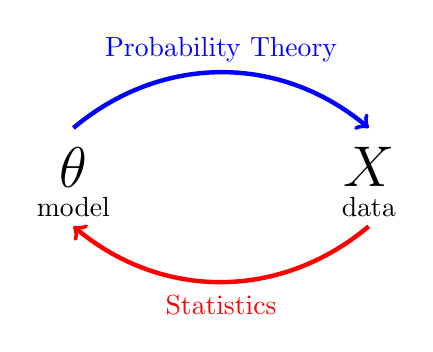
\begin{tikzpicture}[scale=2.5]
    \node [blue] at (0.75, 0.4) {Probability Theory};
    \node [red] at (0.75, -0.9) {Statistics};
    \draw [->,ultra thick,blue] (0,0) to [bend left=40] (1.5,0);
    \draw [->,ultra thick,red] (1.5,-0.5) to [bend left=40] (0,-0.5) ;
    \node at (0,-0.2) {\huge{$ \theta $}};
    \node at (1.5,-0.2) {\huge{$ X $}};
    \node at (0,-0.4) {model};
    \node at (1.5,-0.4) {data};
  \end{tikzpicture}
\end{figure}

To illustrate the difference between probability and statistics, suppose we have a model that can generate $ n $ independent coin flips. A classical probability theory problem would be to calculate the probability of $ k $ heads happening in a row. In this case, the model would be given without data. In the case of statistics, we would only have observed data (e.g. $ k $ heads on $ n $ trials) and the model wouldn't be accessible. A classical statistics problem would be to infer the parameters of a model that explains the observed data (e.g. what is the bias of the coin flip in this example).

\subsection{The Frequentist and the Bayesian}
As stated earlier, the statistics problem is ill-defined. Furthermore, even the meaning of a probability can differ from different philosophical point of views. Two major schools of thought using different meaning of probability have arisen: The Frequentist and the Bayesian.

\begin{enumerate}

  \item The \emph{traditional Frequentist} semantic is the following: 

$ P(X = x) $ represents the limiting relative frequency of observing $ X = x $ if we could repeat an infinite number of i.i.d. experiments.

  \item The \emph{Bayesian semantic} is the following:

$ P(X = x) $ encodes an agent ''belief'' that $ X = x $.

The laws of probability characterize a ''rational'' way to combine ''beliefs'' and ''evidence'' (i.e. observations). This approach has many motivations in terms of gambling, utility, decision theory, etc.

\end{enumerate}


\subsection{The Frequentist interpretation of probability}

To illustrate the view of the Frequentist interpretation, we will analyze an example.
For a discrete random variable, suppose that $ P\{X = x\} = \theta $ then $ P\{X \neq x\} = 1 - \theta $.

Let $ B \triangleq \mathbbm{1}\{ X = x \} \sim \Bern (\theta) $, which encodes the event that $X$ takes the value $x$.

Suppose we repeat the i.i.d. experiments a large number of times, i.e. $ B_i \widesim{iid} \Bern(\theta)$.

By the \emph{law of large numbers}, we have that the empirical average i.i.d. R.V.'s will converge to its expected value: 
$$ \frac{1}{n} \sum_{i} B_i \underset{n \rightarrow \infty}{\rightarrow} \mathbbm{E}\lbrack B_i \rbrack = \theta $$

We can also show that the empirical average will concentrates tightly around the value $\theta$ (by the \emph{central limit theorem}).

Consider the R.V. which represents the sum, it has the distribution:
$$ \sum_{i = 1}^{n} B_i \sim \Bin(n, \theta) $$
The expected value and the variance of the average are the following:
$$ \frac{1}{n} \mathbbm{E} \lbrack \sum_{i} B_i \rbrack = \frac{n \theta}{n} = \theta $$ 
$$ \Var \lbrack \frac{1}{n} \sum_{i} B_i \rbrack = \frac{1}{n^2} \Var \lbrack \Bin(n, \theta) \rbrack = \frac{1}{n^2} n \theta (1 - \theta) = \frac{\theta (1 - \theta)}{n} .$$
We thus see that the variance of the empirical average goes to zero as $n \rightarrow \infty$, showing the concentration.

More precisely, we have by the central limit theorem that:
$$ \sqrt{n} \left( \frac{1}{n} \Bin(n, \theta) - \theta \right) \xrightarrow{d} \mathcal{N}(0, \theta (1 - \theta))) $$
Notice the scaling of the difference by $\sqrt{n}$. For large $n$, the distribution of the empirical average is close to a Gaussian distribution with mean $\theta$ and variance $\theta (1-\theta) / n$.

\subsection{The Bayesian Approach}
The Bayesian approach is very simple philosophically: it treats all uncertain quantities as random variables.

In fact, it encodes all the knowledge about a system (the ''beliefs'') as ''prior'' on probabilistic models and then uses laws of probabilities (and Bayes rule) to get answers.

The simplest example to illustrate the Bayesian approach is the result of $ n $ coin flips of a biased coin. We believe that $ X \sim \Bin(n, \theta) $. Since $ \theta $ is unknown, we model it as a random variable. Thus, we need a ''prior distribution'' $ p(\theta) $ with a sample space defined as $ \Omega_{\Theta} = \lbrack 0,1 \rbrack $.

Suppose we observe $ X = x $ (the result of $ n $ flips), then, we can ''update'' our belief about $ \theta $ using Bayes rule: \footnote{Note that if $ p(x \mid \theta) $ is a pmf and $ p(\theta) $ is a pdf, then the {\it joint} $ p(x , \theta) $ will be a mixed distribution. }

$$ p(\theta \mid X = x) = \frac{p(x \mid \theta) p(\theta)}{p(x)} $$

where,
\begin{itemize}
    \item[] $ p(\theta \mid X = x) $ is the \emph{posterior belief}, 
    \item[] $ p(x \mid \theta) $ is the \emph{likelihood} or the observation model, 
    \item[] $ p(\theta) $ is the \emph{prior belief} and 
    \item[] $ p(x) $ is the \emph{normalization} or ''marginal likelihood''
\end{itemize}



To illustrate the bayesian approach, suppose that $ p( \theta ) $ is a uniform on $ \lbrack 0,1 \rbrack $, i.e. the prior doesn't encode specific preferences.

$$ p(\theta \mid x) \propto \theta^{x} (1 - \theta)^{n - x} \mathbbm{1}_{\lbrack 0, 1 \rbrack}( \theta )$$

(where $ x \in 0:n $) The symbol ''$ \propto $'' means that it is proportional to, i.e. we can drop any term that doesn't contain $ \theta $.

The scaling factor is:

$$ \int_{0}^{1} \theta^x (1 - \theta)^{n - x} \,d\theta = B(x + 1, n - x + 1) $$

The \defobj{beta function} is defined as:
\defmean{ $$ B(a, b) \triangleq \frac{\Gamma(a)\Gamma(b)}{\Gamma(a + b)} $$ }

The \defobj{gamma function} is defined as:
\defmean{ $$ \Gamma (a) \triangleq \int_{0}^{\infty} u^{a - 1} e^{-u} \,du $$ }

$ p(\theta \mid x) = \text{Beta}(\theta ; x + 1, n - x + 1)$ is a \defobj{beta distribution} defined as:
\defmean{ $$ \text{Beta}(\theta; \alpha, \beta) \triangleq \frac{\theta^{\alpha - 1}(1 - \theta)^{\beta - 1}}{B(\alpha, \beta)} \mathbbm{1}_{\lbrack 0,1 \rbrack}(\theta)$$ }

As a Bayesian, the posterior distribution $ p(\theta \mid X = x) $ contains all the information we need to predict the likelihood of an event.

For example, what is the probability that the next coin flip is $ F = 1$? \footnote{By convention, a lowercase $ \theta $ is used even if it's a random variable because $\Theta$ is already used for the parameter space.}

$$ p(F = 1 \mid \theta) = \theta $$

By using the marginalization over $ \theta $, we get:
$$ P(F = 1 \mid X = x) = \int_{\theta} P(F = 1, \theta \mid X = x) \,d\theta$$
By using the chain rule, we get:
$$ = \int_{\theta} P(F = 1 \mid \theta, X = x) P(\theta \mid X = x) \,d\theta $$
Now we have $ P(F = 1 \mid \theta, X = x)= \theta $ by the definition of our model, and thus we get:
$$ \int_{\theta} \theta P(\theta \mid X = x) \,d\theta = \mathbbm{E}_{\theta}\lbrack \theta \mid X = x \rbrack $$
Where the conditional expectation is called the \emph{posterior mean} of $ \theta $.

\noindent A meaningful Bayesian estimator of $ \theta $ is \defobj{$ \hat{\theta}_{Bayes}(x) $} \defmean{$ \triangleq \mathbbm{E}_{\theta}\lbrack \theta \mid X = x \rbrack $}. \footnote{Notation: $ \hat{\theta} $ is a statistical estimator of $ \theta $. Based on the observations, $ \hat{\theta} $ is a value included in the valid set of parameters $ \Theta $. The Frequentist statistics consider multiple possible estimators: MAP, Bayesian posterior mean, MLE, moment matching. After selecting an estimator, we can analyze their statistical properties:
bias, variance, consistency.}

Since $ p(\theta \mid x) $ is a Beta and the expected value of a Beta is:

$$ \mathbbm{E}\lbrack Beta(\theta; \alpha, \beta) \rbrack \triangleq \frac{\alpha}{\alpha + \beta} $$

then the Bayes estimator is:

$$ \mathbbm{E}\lbrack \theta \mid X = x \rbrack = \frac{x + 1}{n + 2} = \hat{\theta}_{Bayes}(x) $$

If we compare it to the ML estimator from the Frequentist approach:

$$ \hat{\theta}_{MLE}(x) = \frac{x}{n} $$

We can see that while the MLE is unbiased, the Bayesian estimator is biased, but asymptotically unbiased. Furthermore, the Bayesian estimator encodes an uncertainty: even if the data contains only head flips, the estimator gives a small probability to flip a tail. This, however, is not the case with the MLE estimator (which tends to overfit).


\end{document}